
\documentclass[12pt, a4paper]{article}
\usepackage{fullpage}
\usepackage{graphicx}
\usepackage{wrapfig}
\usepackage{amsmath}
\usepackage{float}
\usepackage{listings}
\usepackage{lmodern}  % for bold teletype font
\usepackage{xcolor}   % for \textcolor

\definecolor{codegreen}{rgb}{0,0.6,0}
\definecolor{codegray}{rgb}{0.5,0.5,0.5}
\definecolor{codepurple}{rgb}{0.58,0,0.82}
\definecolor{backcolour}{rgb}{0.95,0.95,0.92}

\title{\textbf{EE2703 : Applied Programming Lab \\ Assignment 8}} % Title

\author{Potta Muni Asheesh \\ EE19B048} % Author name

\date{\today} % Date for the report

\begin{document}	
\lstset{
  language=Python,
  backgroundcolor=\color{backcolour},   
  commentstyle=\color{codegreen},
  keywordstyle=\color{magenta},
  numberstyle=\tiny\color{codegray},
  stringstyle=\color{codepurple},
  basicstyle=\ttfamily,
  breakatwhitespace=false,         
  breaklines=true,                 
  captionpos=b,                    
  keepspaces=true,                 
  %numbers=left,                    
  %numbersep=5pt,                  
  showspaces=false,                
  showstringspaces=false,
  showtabs=false,                  
  tabsize=2,
  columns=fullflexible,
  frame=single,
  postbreak=\mbox{\textcolor{red}{$\hookrightarrow$}\space},
}	
		
\maketitle % Insert the title, author and date

\section{Introduction}

In this assignment, circuit analysis using Laplace transforms is done using \texttt{sympy} as a tool for symbolic algebra.

\section{Low pass filter}

The following low pass filter is considered.
\begin{figure}[H]
\centering
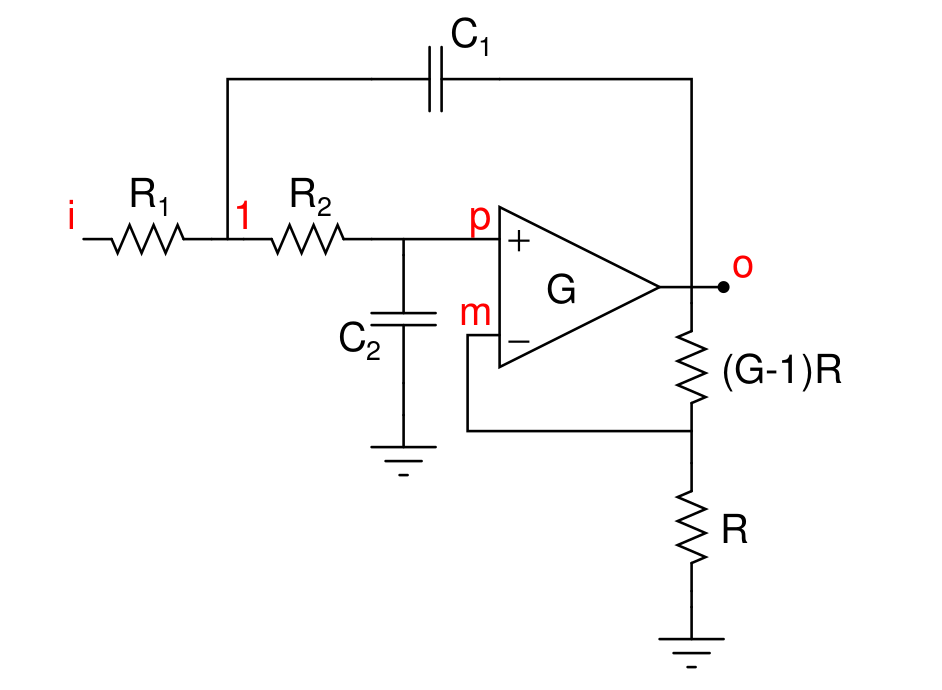
\includegraphics[width=0.8\textwidth]{lowpass.png}
\caption{Circuit diagram of lowpass filter}
\end{figure}
where, the Op-Amp is ideal and $G = 1.586$, $R_1 = R_2  = 10k\Omega$ and $C_1 = C_2 = 10pF$. This gives a second order Butter-worth filter with cutoff frequency of $10/2\pi$MHz.
As the op-amp is considered ideal, the circiut equations are
\begin{equation}
V_m = \frac{V_o}{G}
\end{equation}
\begin{equation}
V_p = \frac{V_1}{1 + sC_2 R_2}
\end{equation}
\begin{equation}
V_p = V_m 
\end{equation}
\begin{equation}
\frac{V_i - V_1}{R_1} + \frac{V_p - V_1}{R_2} + sC_1(V_o - V_i) = 0
\end{equation}

These equations upon solving give the $V_i$ to $V_o$ transfer function as
\begin{equation*}
\frac{V_o}{V_i} = \frac{1.586}{1 + \frac{1.414s}{10^7} + \frac{s^2}{10^{14}}}
\end{equation*}

This circuit analysis is done in python using sympy module.

The four circuit equations are solved by rewriting them as a matrix equation and using sympy to solve the matrix equation.

\begin{equation*}
\left(
\begin{matrix}
0 & 0 & 1 & \frac{-1}{G} \\
\frac{1}{1+sR_2C_2} & -1 & 0 & 0 \\
0 & 1 & -1 & 0 \\
\frac{1}{R_1}+\frac{1}{R_2}+sC_1 & \frac{-1}{R_2} & 0 & -sC_1
\end{matrix}
\right)
\left(
\begin{matrix}
V_1 \\
V_p \\
V_m \\
V_o
\end{matrix}
\right) = 
\left(
\begin{matrix}
0 \\
0 \\
0 \\
\frac{V_i(s)}{R_1}
\end{matrix}
\right)
\end{equation*}

A function is defined in python takes, the circuit parameters and Laplace transform of input signal, as arguments and returns the matrix as \texttt{A}, the input vector as \texttt{b} and the voltage vector as \texttt{V}.

\begin{lstlisting}
import numpy as np
import matplotlib.pyplot as plt
import scipy.signal as sp
import sympy as sym

def lowpass(R1,R2,C1,C2,G,Vi):
    s = sym.symbols('s')
    A = sym.Matrix([[0,0,1,-1/G],[1/(1 + s*C2*R2),-1,0,0],[0,1,-1,0],[1/R1+1/R2+s*C1,-1/R2, 0, -s*C1]])
    b = sym.Matrix([0,0,0,Vi/R1])
    V = A.inv()*b
    return (A, b, V)
\end{lstlisting}

The Frequency response of the low pass filter as obtained by extracting the coefficients of the numerator and the denominator of the rational expression for $V_o$ in the array \texttt{V}. This is done as shown below.
The frequency response obtained is shown below. The DC gain of the filter is $20log(G) = 4dB$.

\begin{figure}[H]
\centering
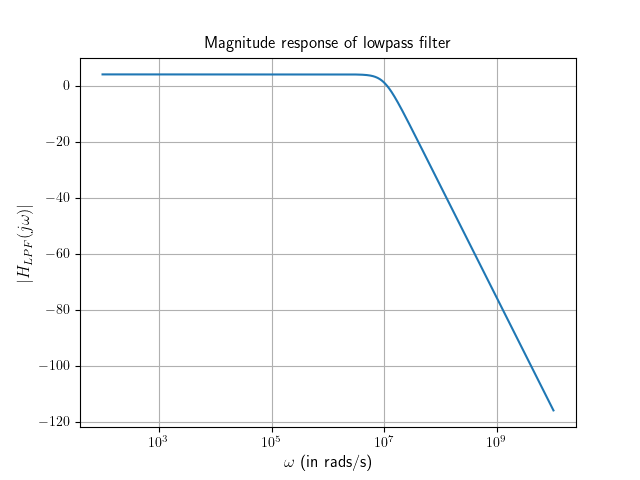
\includegraphics[width=0.8\textwidth]{magResLPF.png}
\caption{Magnitude response of lowpass filter}
\end{figure}

\begin{figure}[H]
\centering
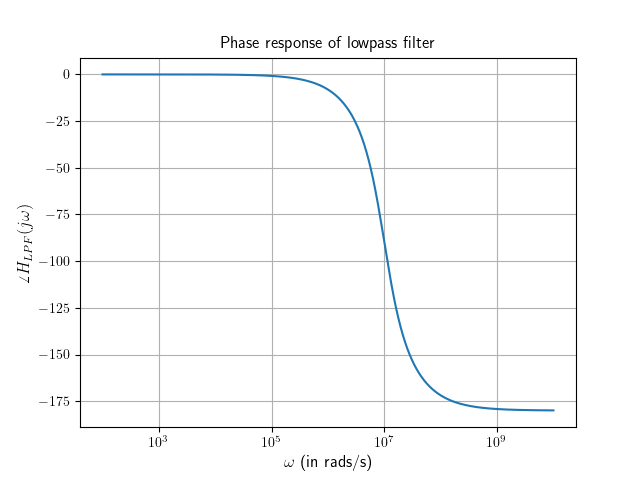
\includegraphics[width=0.8\textwidth]{phaseResLPF.png}
\caption{Phase response of lowpass filter}
\end{figure}

\begin{lstlisting}
def freq_resp_lpf():
    s = sym.symbols('s')
    A, b, V = lowpass(10000, 10000, 1e-11, 1e-11, 1.586, 1)
    Vo = V[3]
    # print(Vo)
    num , den = Vo.as_numer_denom()
    num, den = np.array(sym.Poly(num, s).all_coeffs(), dtype=float), np.array(sym.Poly(den, s).all_coeffs(), dtype=float)
    # num, den = [1.586], [1e-10, 1.414e-5, 1]
    H = sp.lti(num, den)

    global fignum

    plt.figure(fignum)
    fignum += 1
    w = np.logspace(2,10,801)
    w, mag, phi = H.bode(w)
    plt.semilogx(w, mag)
    plt.grid(True)
    plt.title(r'Magnitude response of lowpass filter')
    plt.xlabel(r'$\omega$ (in rads/s)', size=12)
    plt.ylabel(r'$|H_{LPF}(j\omega)|$', size=12)

    plt.figure(fignum)
    fignum += 1
    plt.semilogx(w, phi)
    plt.grid(True)
    plt.title(r'Phase response of lowpass filter')
    plt.xlabel(r'$\omega$ (in rads/s)', size=12)
    plt.ylabel(r'$\angle H_{LPF}(j\omega)$', size=12)
\end{lstlisting}

To get the step response $s(t)$, simply giving $V_i(s) = 1/s$ and using \texttt{impulse} to get the time domain output voltage $v_o(t)$.

\begin{lstlisting}
def q1():
    s = sym.symbols('s')
    A, b, V = lowpass(10000, 10000, 1e-11, 1e-11, 1.586, 1/s)
    Vo = V[3]
    num , den = Vo.as_numer_denom()
    num, den = np.array(sym.Poly(num, s).all_coeffs(), dtype=float), np.array(sym.Poly(den, s).all_coeffs(), dtype=float)
    H = sp.lti(num, den)

    t = np.arange(0, 1e-5, 1e-8)
    t, y = sp.impulse(H, None, t)
    global fignum
    plt.figure(fignum)
    fignum += 1
    plt.plot(t, y)
    plt.title(r'Step response ($s(t)$) of lowpass filter')
    plt.xlabel(r"time $t$ (in seeconds)", size=12)
    plt.ylabel(r'$s(t)$', size=12)
    plt.grid(True)
\end{lstlisting}

\begin{figure}[H]
\centering
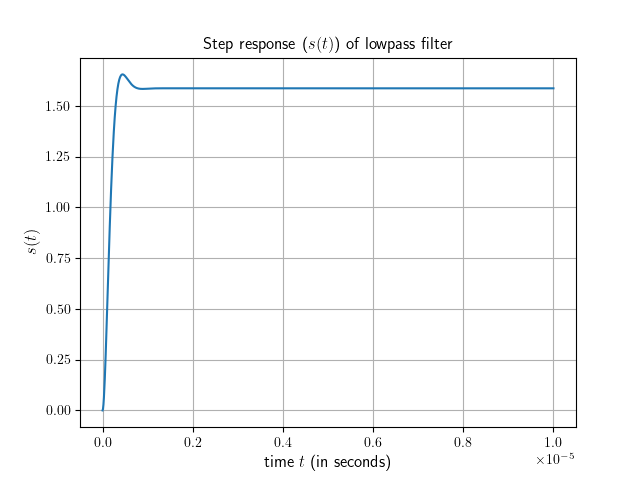
\includegraphics[width=0.8\textwidth]{q1.png}
\caption{Step response of lowpass filter}
\end{figure}

\section{High pass filter}

The following circuit is considered.

\begin{figure}[H]
\centering
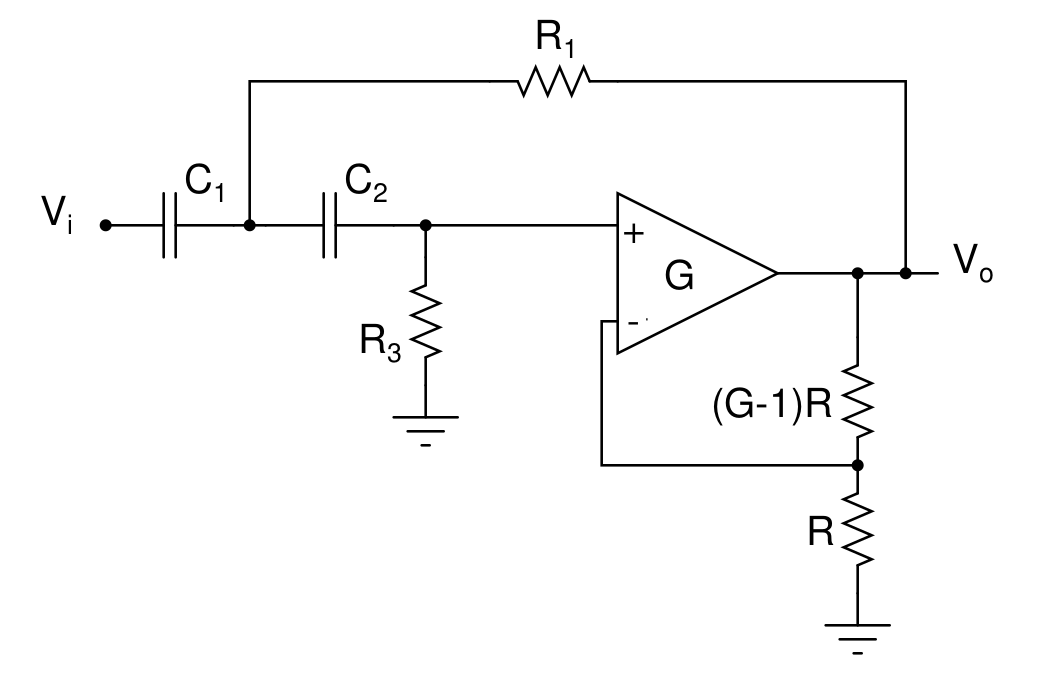
\includegraphics[width=0.7\textwidth]{highpass.png}
\caption{Circuit diagram of high pass filter}
\end{figure}

where, the Op-Amp is ideal and $G = 1.586$, $R_1 = R_3  = 10k\Omega$ and $C_1 = C_2 = 1nF$. This gives a second order Butter-worth filter with cutoff frequency of $1/20\pi$MHz.

As the op-amp is considered ideal, the circiut equations are
\begin{equation}
V_m = \frac{V_o}{G}
\end{equation}
\begin{equation}
V_p = V_1\frac{sC_2R_3}{1 + sC_2 R_3}
\end{equation}
\begin{equation}
V_p = V_m 
\end{equation}
\begin{equation}
(V_i - V_1)sC_1 + (V_p - V_1)sC_2 + \frac{V_o - V_i}{R_1} = 0
\end{equation}

These equations upon solving give the $V_i$ to $V_o$ transfer function as
\begin{equation*}
\frac{V_o}{V_i} = 1.586\frac{\frac{s}{10^{10}}}{1 + \frac{1.414s}{10^5} + \frac{s^2}{10^{10}}}
\end{equation*}

A similar function for highpass filter is also defined.

\begin{lstlisting}
def highpass(R1, R3, C1, C2, G, Vi):
    s = sym.symbols('s')
    A = sym.Matrix([[0,0,1,-1/G],[(s*C2*R3)/(1 + s*C2*R3),-1,0,0],[0,1,-1,0],[1/R1+s*C1+s*C2,-s*C2, 0, -1/R1]])
    b = sym.Matrix([0,0,0,Vi*s*C1])
    V = A.inv()*b
    return (A, b, V)
\end{lstlisting}

When the following input voltage is given at $V_i$
\begin{equation*}
v_i(t) = (sin(2000\pi t) + cos(2 \times 10^6 t))u(t)
\end{equation*}
The transfer function is extracted using sympy and \texttt{lsim} is used to get the output voltage $v_o(t)$. This is done as shown below.

\begin{lstlisting}
def q2():
    s = sym.symbols('s')
    A, b, V = highpass(10000, 10000, 1e-9, 1e-9, 1.586, 1)
    Vo = V[3]
    # print(Vo)
    num , den = Vo.as_numer_denom()
    num, den = np.array(sym.Poly(num, s).all_coeffs(), dtype=float), np.array(sym.Poly(den, s).all_coeffs(), dtype=float)
    H = sp.lti(num, den)

    t = np.arange(0, 10e-3, 1e-7)
    vi = np.sin(2*np.pi*1e3*t) + np.cos(2*np.pi*1e6*t)
    t, vo = sp.lsim(H, vi, t)[:2]
\end{lstlisting}

The plots $v_i(t)$ and $v_o(t)$ for $t < 10\mu s$ and $t < 1ms$ are given below.

\begin{figure}[H]
\centering
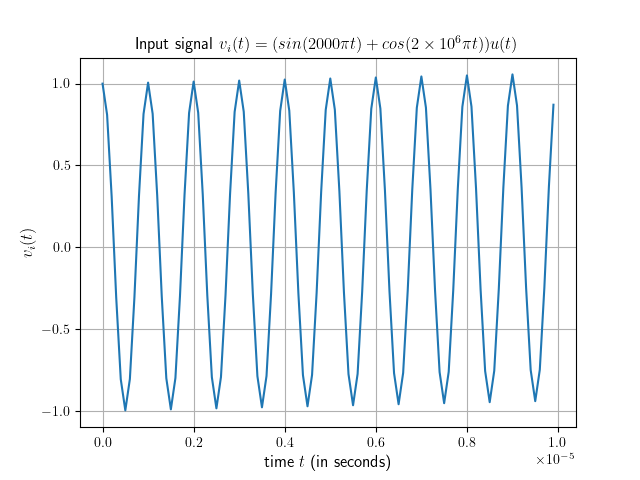
\includegraphics[width=0.8\textwidth]{q2Input1.png}
\caption{Input voltage for $t < 10\mu s$}
\end{figure}

\begin{figure}[H]
\centering
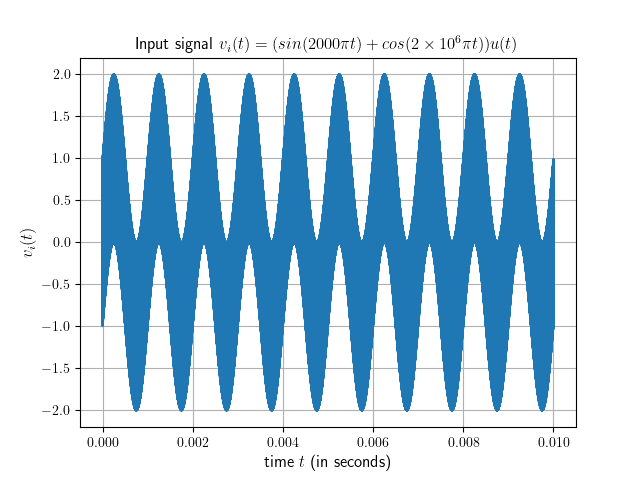
\includegraphics[width=0.8\textwidth]{q2Input2.png}
\caption{Input voltage for $t < 1ms$}
\end{figure}

\begin{figure}[H]
\centering
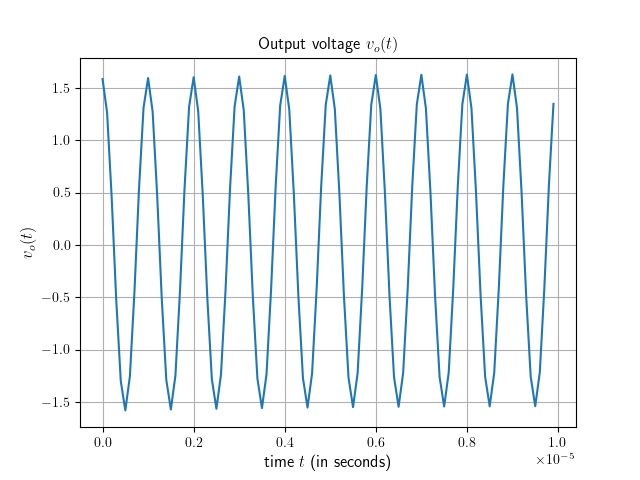
\includegraphics[width=0.8\textwidth]{q2Output1.png}
\caption{Output voltage for $t < 10\mu s$}
\end{figure}

\begin{figure}[H]
\centering
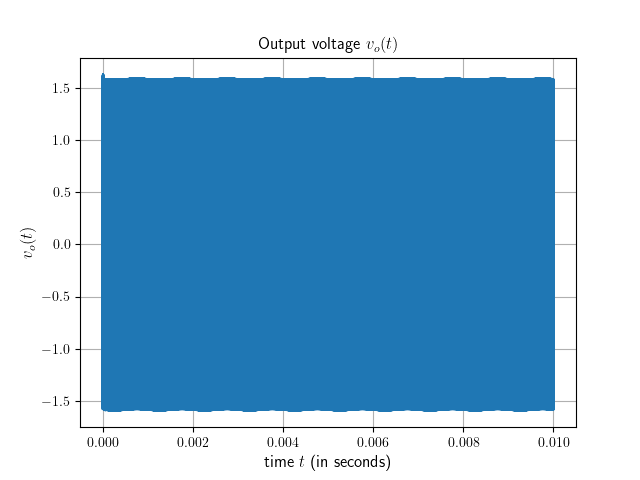
\includegraphics[width=0.8\textwidth]{q2Output2.png}
\caption{Output voltage for $t < 1ms$}
\end{figure}

It can be seen clearly that the lower frequency $\omega = 2000\pi$ component of $v_i$ is attenuated and the higher frequency $\omega = 2\pi \times 10^6$ component is amplified by 1.586 times.

The coefficients of the transfer function obtained using sympy are used to create the system transfer function using \texttt{lti} from \texttt{scipy.signal}.

From this, the frequency response of the system can be obtained. The plots of the frequency response are shown below.

\begin{lstlisting}
def q3():
    s = sym.symbols('s')
    A, b, V = highpass(10000, 10000, 1e-9, 1e-9, 1.586, 1)
    Vo = V[3]
    # print(Vo)
    num , den = Vo.as_numer_denom()
    num, den = np.array(sym.Poly(num, s).all_coeffs(), dtype=float), np.array(sym.Poly(den, s).all_coeffs(), dtype=float)
    H = sp.lti(num, den)

    w = np.logspace(0,8,801)
    w, mag, phi = H.bode(w)
\end{lstlisting}

\begin{figure}[H]
\centering
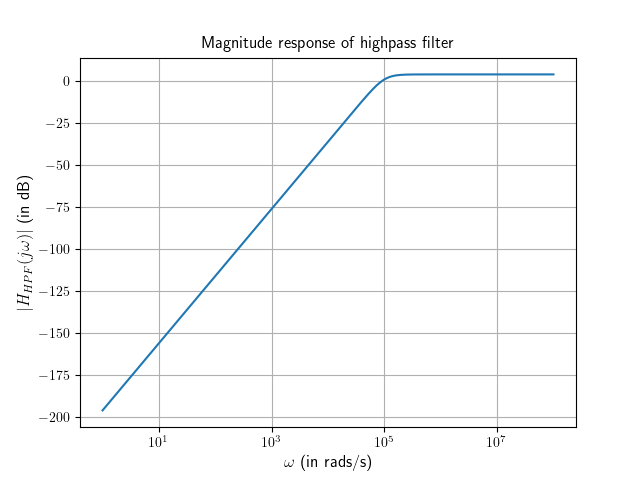
\includegraphics[width=0.8\textwidth]{q3MagHPF.png}
\caption{Magnitude response of high pass filter}
\end{figure}

\begin{figure}[H]
\centering
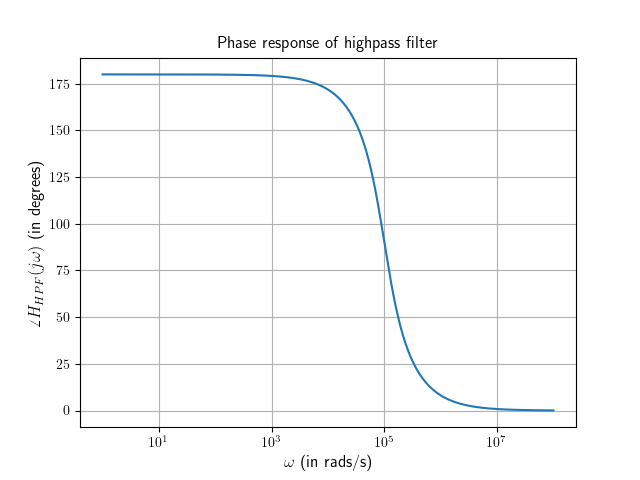
\includegraphics[width=0.8\textwidth]{q3PhaseHPF.png}
\caption{Phase response of high pass filter}
\end{figure}

Consider the input voltage $v_i(t) = exp(-10^4 t)cos(10^7 t)$, then it's laplace transform $V_i(s)$ is given as
\begin{equation*}
V_i(s) = \frac{s+10^4}{(s+10^4)^2 + 10^{14}}
\end{equation*}

This is given as input to the function \texttt{highpass} and the laplace transform of output voltage $v_o(t)$ is obtained. \texttt{impulse} command is used to obtain the time domain signal.

\begin{lstlisting}
def q4():
    s = sym.symbols('s')
    a, w0 = 1e4, 1e7
    Vi = (s+a)/((s+a)**2 + w0**2)
    A, b, V = highpass(10000, 10000, 1e-9, 1e-9, 1.586, Vi)
    Vo = V[3]
    # print(Vo)
    Vi_TF = sp.lti([1, a], [1, 2*a, w0**2 + a**2])
    num , den = Vo.as_numer_denom()
    num, den = np.array(sym.Poly(num, s).all_coeffs(), dtype=float), np.array(sym.Poly(den, s).all_coeffs(), dtype=float)
    H = sp.lti(num, den)

    t = np.arange(0, 1e-4, 1e-8)
    vi = np.exp(-a*t)*np.cos(w0*t)
    t, h = sp.impulse(H, None, t)
\end{lstlisting}

\begin{figure}[H]
\centering
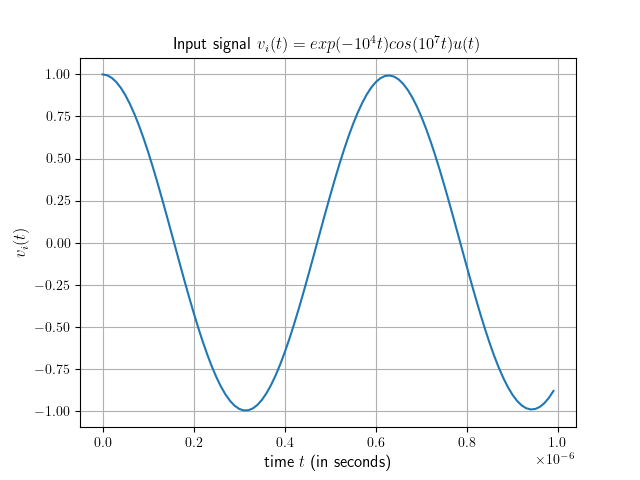
\includegraphics[width=0.8\textwidth]{q4Input1.png}
\caption{Input volatge for $t < 1 \mu s$}
\end{figure}

\begin{figure}[H]
\centering
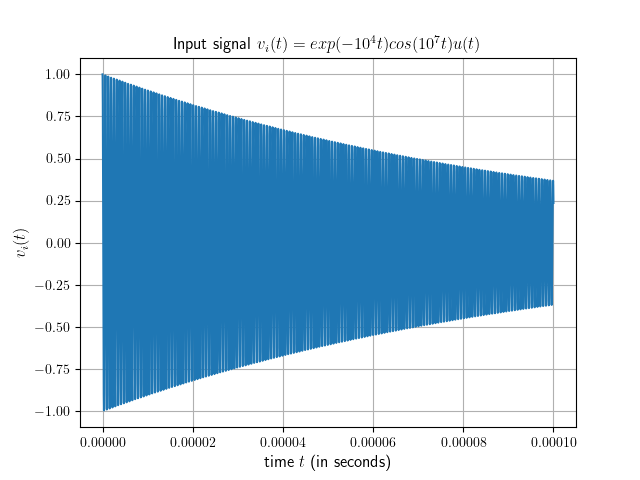
\includegraphics[width=0.8\textwidth]{q4Input2.png}
\caption{Input volatge for $t < 100 \mu s$}
\end{figure}

\begin{figure}[H]
\centering
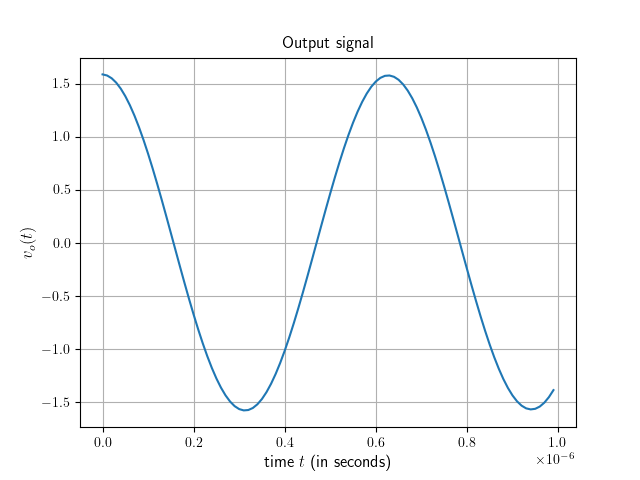
\includegraphics[width=0.8\textwidth]{q4Output1.png}
\caption{Output volatge for $t < 1 \mu s$}
\end{figure}

\begin{figure}[H]
\centering
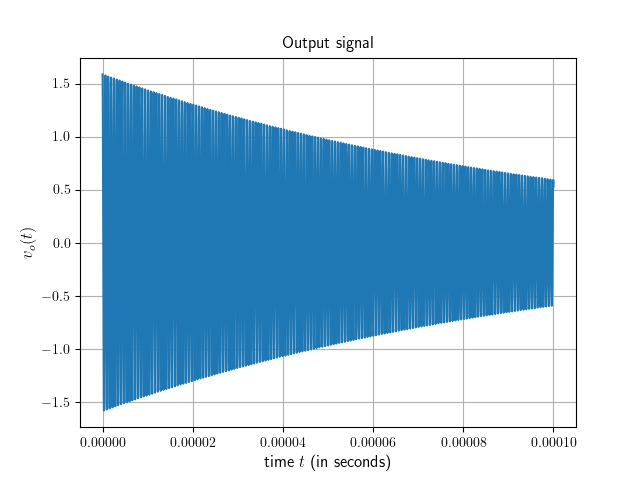
\includegraphics[width=0.8\textwidth]{q4Output2.png}
\caption{Output volatge for $t < 100 \mu s$}
\end{figure}

It can be seen that the signal is amplified by 1.586 times.

When the input voltage given is $v_i(t) = exp(-10 t)cos(10^3 t)$, then the laplace transform $V_i(s)$ is given by

\begin{equation*}
V_i(s) = \frac{s+10}{(s+10)^2 + 10^{6}}
\end{equation*}

The output voltage signal is obtained similarly. 

\begin{lstlisting}
def q4():
    s = sym.symbols('s')
    a, w0 = 1e1, 1e3
    Vi = (s+a)/((s+a)**2 + w0**2)
    A, b, V = highpass(10000, 10000, 1e-9, 1e-9, 1.586, Vi)
    Vo = V[3]
    # print(Vo)
    Vi_TF = sp.lti([1, a], [1, 2*a, w0**2 + a**2])
    num , den = Vo.as_numer_denom()
    num, den = np.array(sym.Poly(num, s).all_coeffs(), dtype=float), np.array(sym.Poly(den, s).all_coeffs(), dtype=float)
    H = sp.lti(num, den)

    t = np.arange(0, 1, 1e-4)
    vi = np.exp(-a*t)*np.cos(w0*t)
    t, h = sp.impulse(H, None, t)
\end{lstlisting}

\begin{figure}[H]
\centering
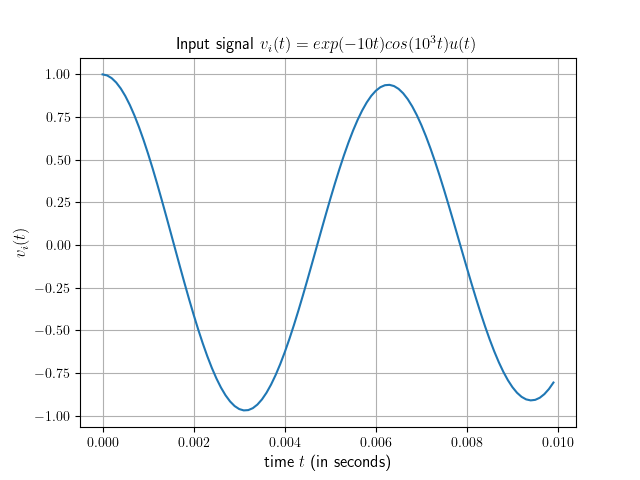
\includegraphics[width=0.8\textwidth]{q4Input3.png}
\caption{Input volatge for $t < 10 ms$}
\end{figure}

\begin{figure}[H]
\centering
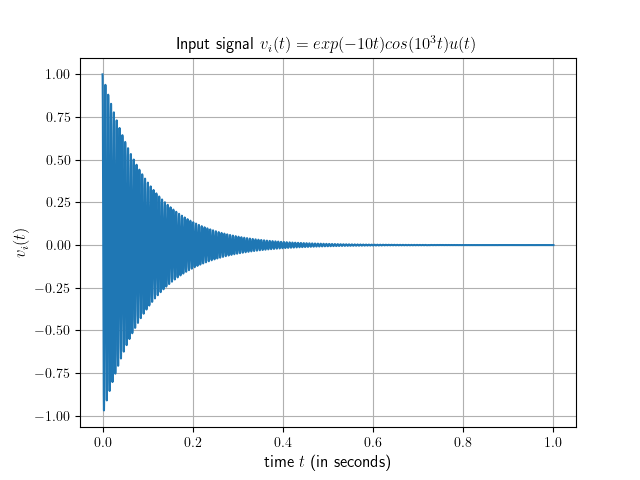
\includegraphics[width=0.8\textwidth]{q4Input4.png}
\caption{Input volatge for $t < 1 s$}
\end{figure}

\begin{figure}[H]
\centering
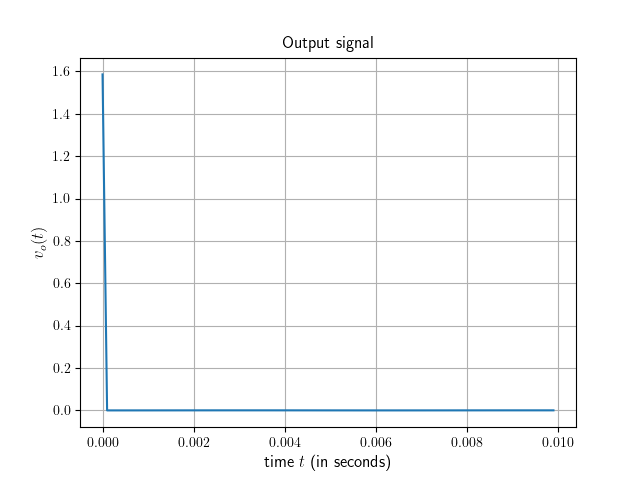
\includegraphics[width=0.8\textwidth]{q4Output3.png}
\caption{Output volatge for $t < 10 ms$}
\end{figure}

\begin{figure}[H]
\centering
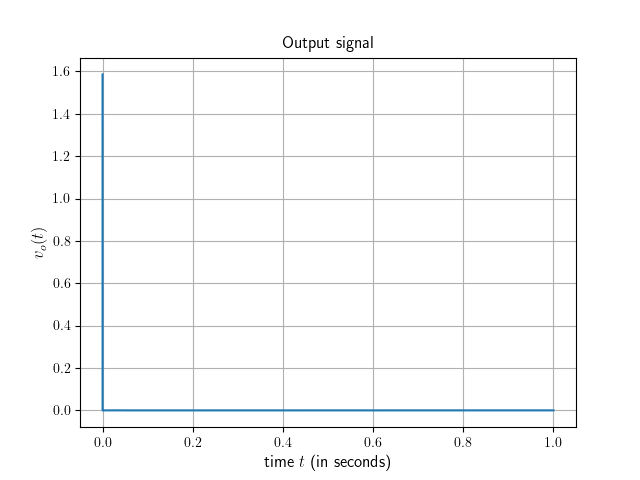
\includegraphics[width=0.8\textwidth]{q4Output4.png}
\caption{Output volatge for $t < 1 s$}
\end{figure}

It can be seen that the signal is attenuated.

Similarly, to get the step response, the laplace transform of input is given as $V_i(s) = 1/s$ to the function \texttt{highpass} to get the laplace transform of output voltage signal.

\begin{lstlisting}
def q5():
    s = sym.symbols('s')
    A, b, V = highpass(10000, 10000, 1e-9, 1e-9, 1.586, 1/s)
    Vo = V[3]
    # print(Vi)
    # Vi_TF = sp.lti([1, 0.01],[1, 2e-2, 1e7])
    num , den = Vo.as_numer_denom()
    num, den = np.array(sym.Poly(num, s).all_coeffs(), dtype=float), np.array(sym.Poly(den, s).all_coeffs(), dtype=float)
    H = sp.lti(num, den)

    t = np.arange(0, 1e-3, 1e-7)
    t, h = sp.impulse(H, None, t)
\end{lstlisting}

\begin{figure}[H]
\centering
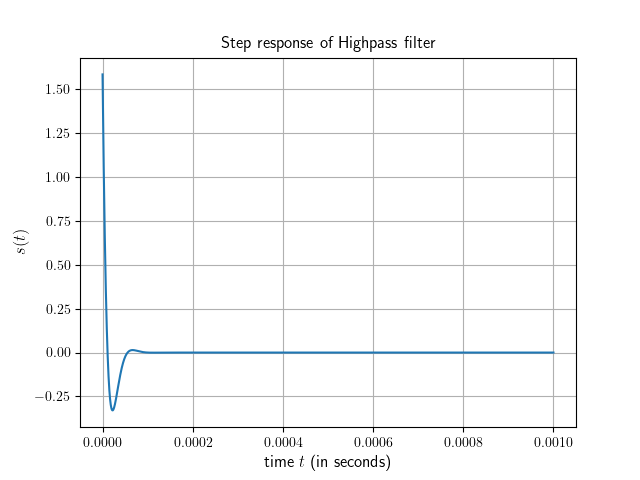
\includegraphics[width=0.8\textwidth]{q5.png}
\caption{Step response of high pass filter}
\end{figure}

\end{document} 
